\chapter{Apéndice}\label{ch:Ap}

\section{Demostraciones del texto}
\subsection{Solución de un sistema lineal}
Se anexa la demostración al \textbf{Teorema 1} [\ref{teo:Solgral}]:
\begin{proof}
	Se propone la función general $X(t)=e^{\lambda t}\vec{v}_0$. Entonces derivamos la función con respecto del tiempo
	\begin{align*}
		\dot{X}(t) &= \lambda e^{\lambda t}\vec{v}_0\\
				   &= e^{\lambda t}(\lambda\vec{v}_0)\\
				   &= e^{\lambda t}(A\vec{v}_0)		\\
				   &= A(e^{\lambda t}\vec{v}_0)\\
				   &= AX(t)
	\end{align*}
\end{proof}

\subsection{Solución de la ecuación logística}\label{sec:SolEqLogistica}

La ecuación logística (\ref{eqn:EqLogistica}) es de las pocas ecuaciones no lineales de las que podemos hallar una solución analítica única. A continuación nos adentraremos a hallar dicha solución. Reescribimos la ecuación de la siguiente manera
$$\frac{dN}{dt}=\frac{rN(K-N)}{K}$$
se utiliza la separación de variables para poder resolver la ecuación, re acomodando nos queda como
$$\frac{KdN}{N(K-N)}=rdt\qquad\Longleftrightarrow\qquad \int\frac{KdN}{N(K-N)}=\int rdt$$
El lado izquierdo lo resolvemos por fracciones parciales, se encomienda al lector comprobar que la siguiente igualdad es verdadera
$$\frac{K}{N(N-K)}=\frac{1}{N}+\frac{1}{K-N}$$
entonces las integrales ya resueltas nos quedan de la siguiente manera
\begin{align*}
	\ln N-\ln(K-N)&=rt+c \\
	\ln\left (\frac{N}{K-N}\right ) &= rt+c\\
	\frac{N}{K-N}&=e^{rt+c}\\
	N&=(K-N)Ce^{rt}\\
	N(1+Ce^{rt})&=KCe^{rt}\\
	N(t)&=\frac{KCe^{rt}}{1+Ce^{rt}}
\end{align*}
Resolviendo el problema de condición inicial se establece que para $t=0$ se tiene $N(0)=N_0$, por tanto la constante $C$ nos queda como
$$C=\frac{N_0}{K-N_0}$$
Finalmente reajustando y acomodando términos, la solución de la ecuación logística es:
\begin{equation}\label{eqn:SolEqLogistica}
	N(t)=\frac{KN_0e^{rt}}{(K-N_0)+N_0e^{rt}}
\end{equation}
Comparado con la solución numérica se ve de la siguiente forma
\begin{figure}[h!]
	\centering
	\includegraphics[scale=0.23]{../Imagenes/Ecuacion Logistica Analítica}
	\caption{Ecuación logística con una tasa de crecimiento $r=2$ y una capacidad de carga $K=10$, se grafica para las mismas condiciones iniciales; (\textbf{A}) Solución analítica. (\textbf{B}) Solución numérica.}
	\label{fig:EcuacionLogisticaAnalitica}
\end{figure}
\newpage
\subsection{Solución del sistema presa-depredador}\label{sec:SolPresaDepredador}

El sistema (\ref{eqn:PresaDepredador}) tiene la dicha de poderse resolver de forma analítica al igual que la ecuación logística y se verá a continuación el procedimiento. Para ello definimos la siguiente regla de la cadena para $y(t)$
$$\frac{dy}{dt} = \frac{dy}{dx}\cdot\frac{dx}{dt}\qquad\Longleftrightarrow\qquad\frac{dy}{dx}=\frac{\frac{dy}{dt}}{\frac{dx}{dt}}$$
sustituyendo las ecuaciones de (\ref{eqn:PresaDepredador}) en $\frac{dy}{dx}$ se tiene
\begin{align*}
	\frac{dy}{dx}&=\frac{\delta xy-\gamma y}{\alpha x-\beta xy}  \\
\end{align*}
Se factoriza lo necesario y se aplica separación de variables para poder integrar las ecuaciones y hallar las soluciones
\begin{align*}
	x(\alpha-\beta y)\, dy &= y(\delta x-\gamma)\, dx\\
	\int \frac{\alpha-\beta y}{y}\, dy &= \int \frac{\delta x-\gamma}{x}\, dx \\
\end{align*}
al integrar finalmente tenemos la solución implícita:
\begin{equation}\label{eqn:CurvasNivelPD}
	f(x,y)=\alpha\ln y+\gamma\ln x-\beta y- \delta x=c
\end{equation}
Ahora veamos las curvas de nivel de la solución analítica en contraste con el espacio fase generado a través de las ecuaciones de (\ref{eqn:PresaDepredador}):
\begin{figure}[h!]
	\centering
	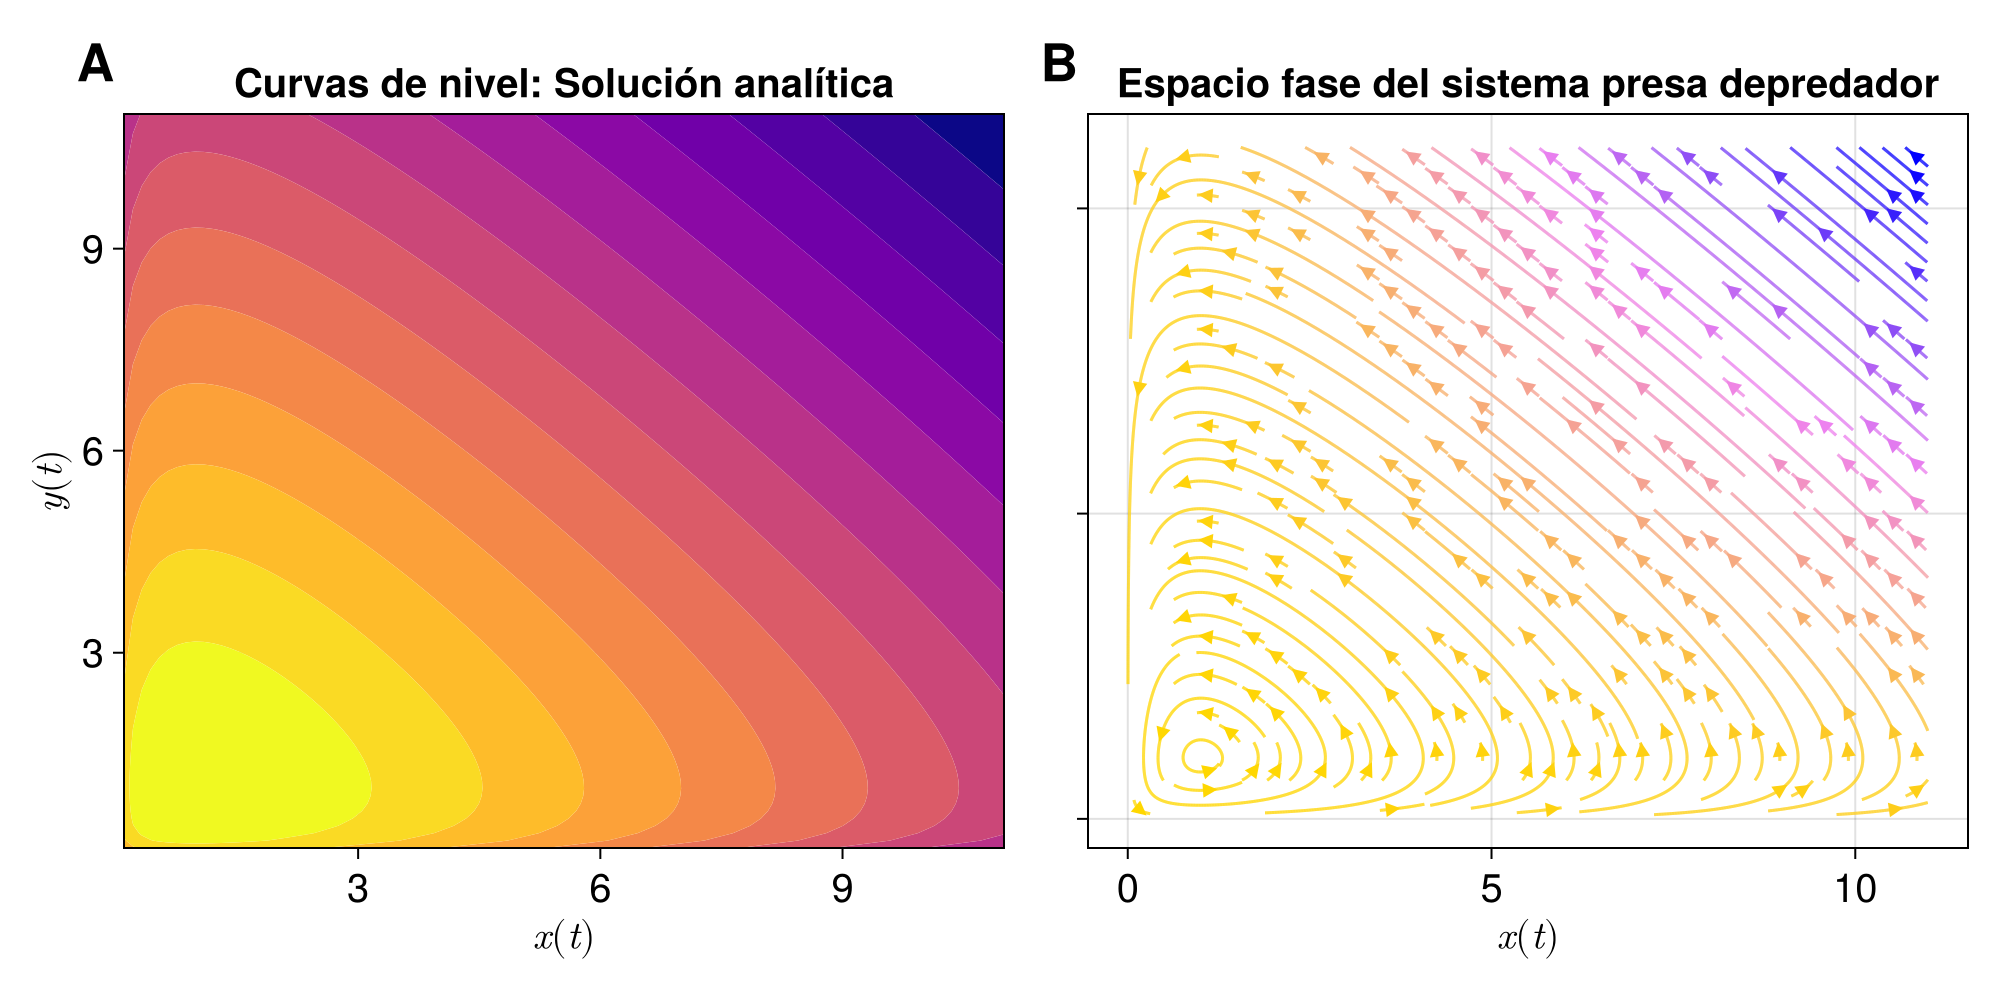
\includegraphics[scale=0.22]{../Imagenes/Curvas de nivel PD}
	\caption{(\textbf{A}) Curvas de nivel utilizando la solución analítica (\ref{eqn:CurvasNivelPD}). (\textbf{B}) Espacio fase generado a partir de las ecuaciones de (\ref{eqn:PresaDepredador}).}
	\label{fig:CurvasNivelPD}
\end{figure}
\newpage
Por último realicemos una rápida comparativa entre los métodos de integración de RK4 y Euler para poder visualizar la razón principal por la que se ha escogido RK4 como método de integración para los sistemas no lineales de esta tesis
\begin{figure}[h!]
	\centering
	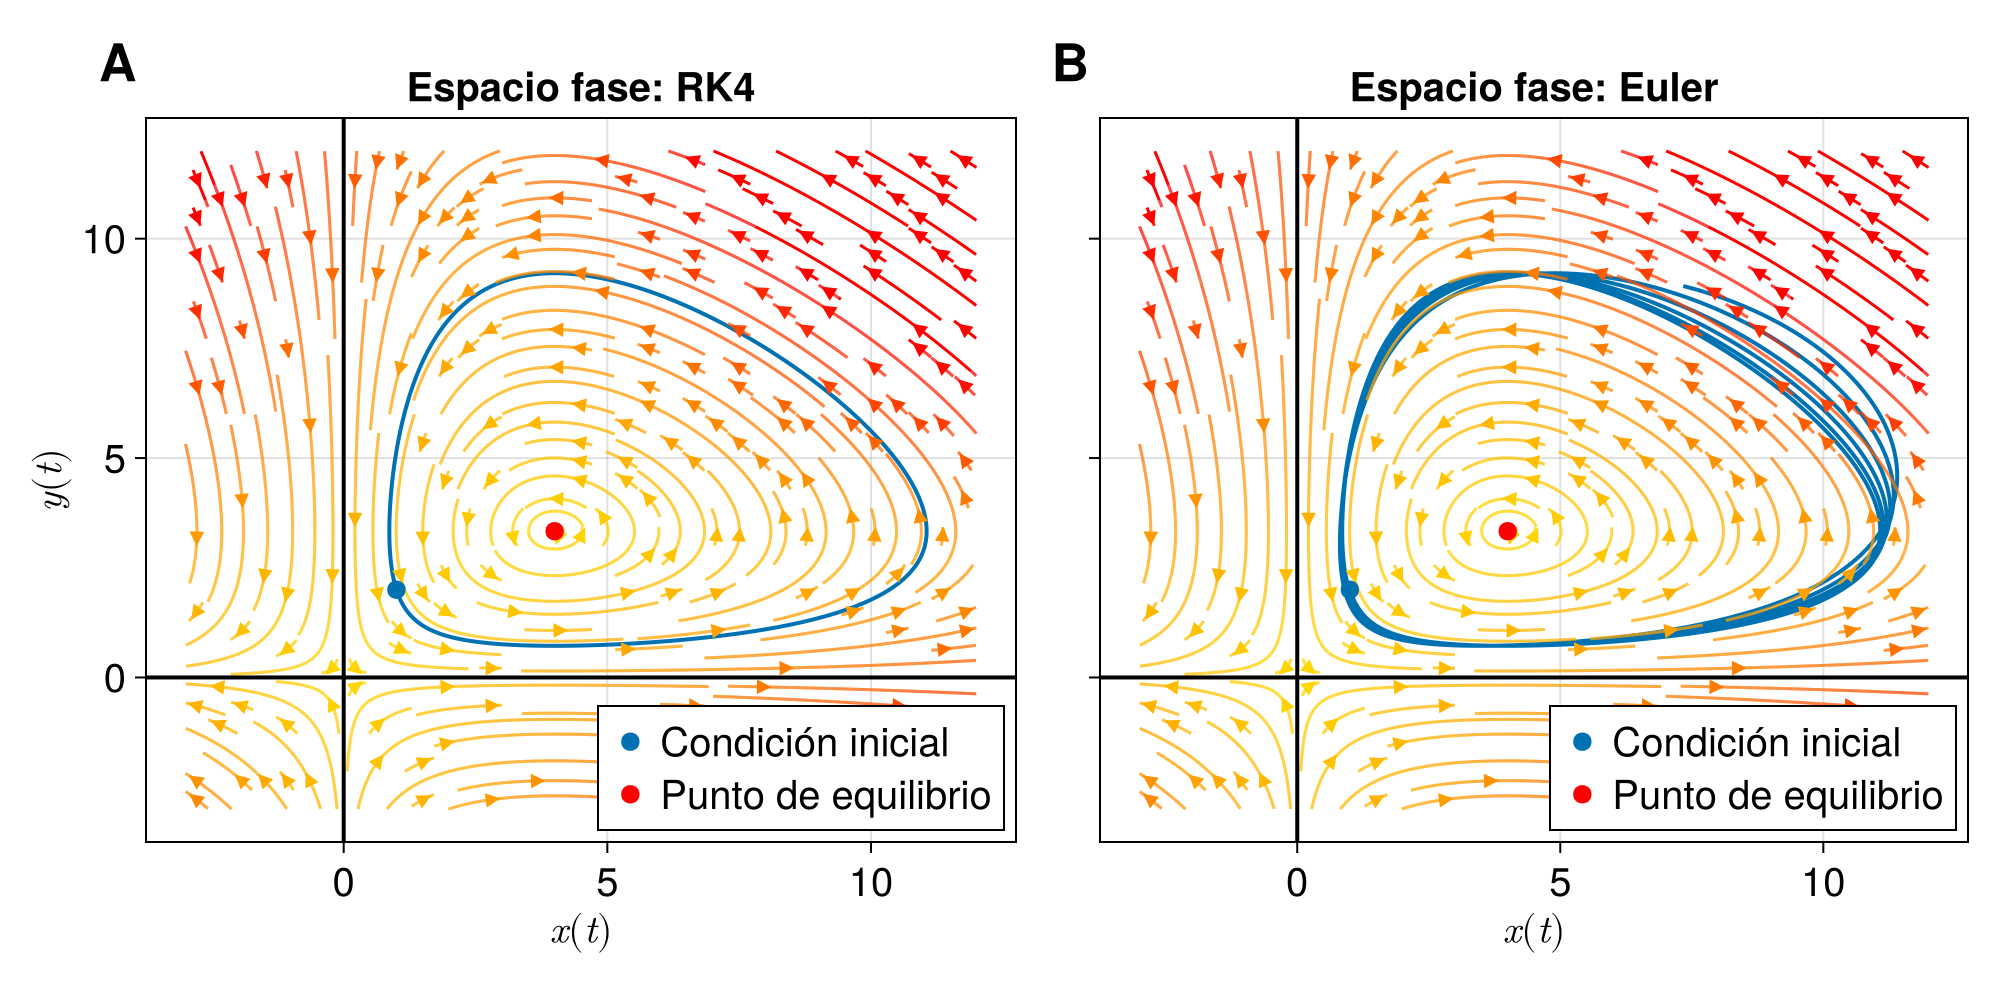
\includegraphics[scale=0.23]{../Imagenes/RK4vsEuler}
	\caption{En ambos ejemplos se integró para $t\in[0,20]$ con un paso de integración de $h=0.01$. (\textbf{A}) Integración del sistema (\ref{eqn:EgPresaDepredador}) con el método de Runge-Kutta orden 4. (\textbf{B}) Integración del sistema (\ref{eqn:EgPresaDepredador}) con el método de Euler.}
	\label{fig:Rk4vsEuler}
\end{figure}

Para fines prácticos, en la siguiente sección se introducen la implementación de ambos métodos en el lenguaje de programación \julia.

\section{Algoritmos y códigos}

\subsection{Códigos para generar imágenes}
El trabajo presente se ha realizado bajo algoritmos hecho en el lenguaje de programación \julia. En esta sección como en otras se estará anexando código en referencia a elementos presentes en el cuerpo de la tesis. Se anexa código de las figuras de los espacios fase de la sección (\ref{sec:Espacios fase}). Cabe mencionar que el motor de graficación utilizado es \href{https://github.com/JuliaPlots/CairoMakie.jl}{\texttt{CairoMakie}} que es ampliamente utilizado para publicaciones científicas por su elegancia, estética y estilo. Se espera que con los bloques de códigos anexados se pueda dar una idea de su uso para su implementación propia del lector.\\
\\
El bloque de código (\ref{al:EspaciosFase}) funciona para generar la Figura (\ref{fig:EFReales}); sin embargo se puede modificar convenientemente para poder generar todos los espacios fase que se presentan a lo de la tesis, únicamente hay que definir las respectivas funciones del sistema para que se pueda generar el campo de direcciones apropiado.
\begin{algorithm}
	\caption{Generación de gráficas de espacios fase de $2\times 2$ con eigenvalores reales usando CairoMakie.}
	\KwData{Matrices de coeficientes.}
	\KwResult{Espacios fase.}
	\label{al:EspaciosFase}
	Inicializar el proceso\;	
	\begin{minted}{julia}
using CairoMakie
xlim = (-3,3)	#Se establecen los límites que abarcarán las gráficas
ylim = (-3,3)

fSilla(X) = Point2(-3X[1],2X[2])  #Se definen las matrices de coeficientes
fAtractor(X) = Point2(-X[1],-4X[2])  #de los sistemas lineales
fRepulsor(X) = Point2(2X[1]+2X[2],X[1]+3X[2])

titles = ["Atractor","Punto silla", "Repulsor"] #Títulos para cada gráfica
functions = [fAtractor,fSilla,fRepulsor]  #Arreglo de funciones para poder iterarlas
n = length(functions)  #más adelante

#Se definen los colores de las líneas de flujo del espacio fase
cmaps = [[:red,:orange,:brown],[:red,:orange,:brown],[:red,:orange,:brown]]

#1. Se define la figura en sus dimensiones y el tamaño de letra.
#2. Se definen los ejes y la información que llevará con ellos. 
#3. Se definen las líneas de campo
#4. Escondemos las y(t) para la figura de en medio y la de la derecha
#5. Se establecen los límites de cada gráfico
fig = Figure(size = (1000, 400), fontsize = 20)
axs = [Axis(fig[1, i], xlabel = "x(t)", ylabel = "y(t)", title = titles[i],
aspect = 1, backgroundcolor = :white) for i in 1:n]
[streamplot!(axs[i], functions[i], -4 .. 4, -4 .. 4, colormap = cmaps[i],
gridsize = (32, 32), arrow_size = 9) for i in 1:n, density = 0.1]
[hideydecorations!(axs[i], grid = false, ticks = false) for i in 2:n]
[limits!(axs[i], xlim...,ylim...) for i in 1:n]
fig	#Se imprime la figura
	\end{minted}
	 Ejecutar el código y obtener el resultado\;
\end{algorithm}

\subsection{Algoritmos}\label{sec:algoritmos}

\subsubsection{Método de Euler}

Aunque no ha sido utilizado este método para la generación de resultados, se cree que es importante agregarlo para aquel que quiera implementarlo por su cuenta y usarlo. Es un método que se generaliza $N$ ecuaciones diferenciales
\begin{algorithm}
	\caption{Método de Euler generalizado}
	\label{al:Euler}
	\begin{minted}{julia}
""" Integrador de Euler generalizado.
f := Función N-dimensional del sistema a integrar
x0 := Condición inicial de
t0 := Tiempo inicial
tf := Tiempo final
dt := Paso de integración """
function eulerND(f::Function,x0::Vector,t0::Int64,tf::Int64,dt::Float64)          
	tiempos = range(t0, stop = tf, step = dt)
	n = length(tiempos)                      
	dim = length(x0)                         
	xs = zeros(n,dim)                        
	xs[1,:] = x0                             
	for i in 2:n 
		xs[i,:] = xs[i-1,:] + dt*f(xs[i-1,:])
	end
	return (tiempos,xs)
end
	\end{minted}
	Explicación del código:\\
	\texttt{range()} es una función que genera una partición para una cota inferior, otra superior y un paso de partición. Se obtiene el tamaño de ese conjunto mediante el efecto de \texttt{lenght()}. Se define la dimensión del sistema aplicando esta misma función pero a la condición inicial \texttt{x0}, esto es importante porque a partir de aquí se va a definir el conjunto solución \texttt{xs} que es una matriz de ceros con \texttt{n} filas y \texttt{dim} columnas: cada columna va a ser la solución numérica de cada ecuación del sistema. Pero antes de comenzar a integrar \texttt{xs[1,:] = x0} posiciona la condición inicial. Posteriormente se realiza un ciclo \texttt{for} de \texttt{2} a \texttt{n} donde se aplica la regla de Euler (\ref{eqn:Euler}). Finalmente se regresa el conjunto de \texttt{tiempos} y la solución N-dimensional \texttt{xs}.
\end{algorithm}
\newpage
Es importante resaltar el uso de \textit{pre-alocación} del arreglo solución, esto agiliza tiempos de ejecución al definir cada uno de los espacios donde irá cada término de la solución, a diferencia de si se ocupa el método \ttt{push!()} (análogo con el \ttt{append()} de python) para ir agregando cada término al arreglo. Esta misma filosofía servirá para la implementación de RK4, lo único que cambiará es la definición de lo que se pone dentro del ciclo \ttt{for}.
\subsubsection{Método de Runge-Kutta 4}

\begin{algorithm}
	\caption{Método de Runge-Kutta 4}
	\label{al:RK4}
	\begin{minted}{julia}
""" Integrador de Euler generalizado.
f := Función N-dimensional del sistema a integrar
x0 := Condición inicial de
t0 := Tiempo inicial
tf := Tiempo final
dt := Paso de integración """
function RK4(f::Function,x0::Vector,t0::Int64,tf::Int64,h::Float64)          
	t = range(t0, stop = tf, step = h)
	n = length(t)
	dim = length(x0)
	xs = zeros(n,dim)
	xs[1,:] = x0
	for i in  2:n
		k1 = f(xs[i-1,:])
		k2 = f(xs[i-1,:]+(h/2)*k1)
		k3 = f(xs[i-1,:]+(h/2)*k2)
		k4 = f(xs[i-1,:]+h*k3)
		xs[i,:] = xs[i-1,:] + (h/6)*(k1+2*k2+2*k3+k4)
	end
	return (t , xs)
end
	\end{minted}
	La única diferencia con respecto al algoritmo (\ref{al:Euler}) es la definición del las reglas dadas por (\ref{eqn:RK4}). En final la función regresa los tiempos de integración \ttt{t} y el arreglo solución N-dimensional \ttt{xs}.
\end{algorithm}

Una vez definidos ambos sistemas tenemos el poder de integrar cualquier sistema de ecuaciones diferenciales lineales y por su puesto: no-lineales. Todo esta en la forma de definir las funciones \ttt{f} N-dimensionales de cada método. Un ejemplo de uso sería el siguiente
\begin{minted}{julia}
#Se define la función N-dimensional
presaDepredador(X::Vector) = [2X[1]-0.6X[1]X[2],0.5X[1]X[2]-2X[2]]
x0 =[1,2]
t0 = 0
tf = 20
h = 0.001
t,xs = RK4(presaDepredador,x0,t0,tf,h)
tE,xsE = eulerND(presaDepredador,x0,t0,tf,h)
\end{minted}
En este caso \ttt{presaDepredador(X::Vector)} (en referencia al sistema (\ref{eqn:EgPresaDepredador})) es la función N-dimensional que ocupará \ttt{eulerND} y \ttt{RK4}. Se define en función de un vector \ttt{X} y devuelve un arreglo de dos entradas donde cada entrada constituye una ecuación del sistema a integrar. Con dichos arreglos solución se pueden graficar las series de tiempo (en función de \ttt{(t,xs[:,i])} con \ttt{i=\{1,2\}}) o los espacios fase (en función de \ttt{(xs[:,1],x[:,2])}).